\documentclass[tikz]{standalone}
\begin{document}
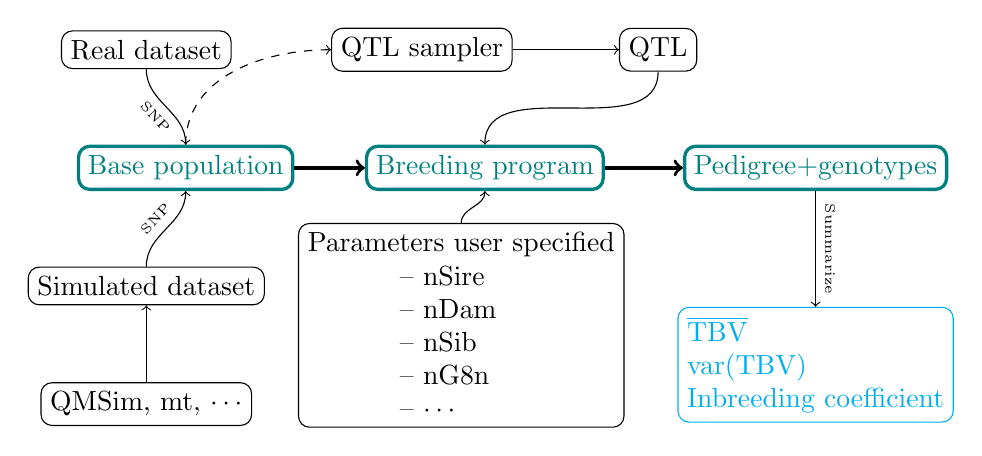
\begin{tikzpicture}
  % \draw[help lines] (0,0) grid (12, 6);
  % \foreach \x in {0, 1, ..., 11} \node[below, gray!50] at (\x,0){\tiny{\x}};
  % \foreach \y in {1, 2, ..., 6} \node[left, gray!50] at (0,\y){\tiny{\y}};
  \node at (2, 3.5) [teal, very thick, rectangle, rounded corners, draw]
  (x) {Base population};
  \node at (5.8, 3.5) [teal, very thick, rectangle, rounded corners, draw]
  (y) {Breeding program};
  \node at (10, 3.5) [teal, very thick, rectangle, rounded corners, draw]
  (rst) {Pedigree+genotypes};
  \node at (1.5, 5) [rectangle, rounded corners, draw] (r) {Real dataset};
  \node at (5, 5) [rectangle, rounded corners, draw] (q) {QTL sampler};
  \node at (8, 5) [rectangle, rounded corners, draw] (qtl) {QTL};
  \node at (1.5, 2) [rectangle, rounded corners, draw] (s) {Simulated dataset};
  \node at (1.5, .5) [rectangle, rounded corners, draw] (p) {QMSim, mt, $\cdots$};
  node[below] {Parameters} 
  \node at (5.5, 1.5) [rectangle, rounded corners, align=left, draw] (par) {Parameters user specified\\ $\qquad\quad$ -- nSire\\ $\qquad\quad$ -- nDam\\ $\qquad\quad$ -- nSib\\ $\qquad\quad$ -- nG8n\\ $\qquad\quad$ -- $\cdots$};
  \node at(10, 1) [cyan, align=left, rectangle, rounded corners, draw] (sum) {$\overline{\mathrm{TBV}}$\\ var(TBV)\\ Inbreeding coefficient};

  \draw[->] (r) to[out=270, in=90] node[below, sloped]{\tiny SNP} (x);
  \draw[->] (s) to[out=90, in=270] node[above, sloped]{\tiny SNP} (x);
  \draw[->] (p) to (s);
  \draw[->, very thick] (x) to (y);
  \draw[->, dashed] (x) to[out=90, in=180] (q);
  \draw[->] (par) to[out=90, in=270] (y);
  \draw[->] (q) -- (qtl);
  \draw[->] (qtl) to[out=270, in=90] (y);
  \draw[->, very thick] (y) -- (rst);
  \draw[->] (rst) to[out=270, in=90] node[above, sloped]{\tiny Summarize} (sum);
\end{tikzpicture}
\end{document}
